\chapter{插值 POD 方法}
\label{cha:sysu-thesis-latex-install-guide}
本征正交分解(Proper Orthogonal Decomposition, POD)方法在流场计算中的应用通常使通过将流动控制方程投影至POD基底空间,实现对原方程系统的降阶建模,最终获得低阶非线性控制方程。该方法在翼型气动优化设计及多学科耦合优化领域已展现出显著工程价值。近年来发展的插值POD方法通过建立扰动参数与基函数系数的映射关系,进一步提升了非设计点流场近似解的求解效率。
\section{插值POD方法}
POD方法的核心在于构造反映物理场特征的本征模态。其采样解集通过系统性地扰动关键物理参数获得,在流体力学应用中,典型扰动变量包括时间步长、迎角、马赫数、翼型几何参数等单因素或多因素耦合变量。由此构建的POD基底具有完备性特征,可表征目标参数扰动域内任意物理状态的流场分布。

根据公式(2-2),每个解都对应一组基系数,采样解也同样对应一组基系数。若扰动变量与基系数之间存在连续的函数关系,则可以根据三次样条插值,利用采样解的扰动变量与基系数,求得扰动范围内的任意扰动情况下的物理解。设有 \(n\) 个扰动变量,每个扰动变量变化 \(m\) 次,计算过程如下:
\begin{enumerate}
    \item 确定扰动变量 \(\delta_j^{(i)}\)(\(j = 1, 2, \ldots, n\)),并由该扰动变量获得一组采样解 \(\{\mathbf{U}_i\}_{i=1}^m\);
    
    \item 由采样解 \(\{\mathbf{U}_i\}_{i=1}^m\) 计算 POD 基 \(\{\Phi^i\}_{i=1}^m\);
    
    \item 用所求的基表达采样解,一般使用一部分基就可以获得很好的表达效果:\(\mathbf{U}^i = \sum_{j=1}^r \alpha_j^i \Phi^j\)(\(p < m \times n\)),对应的基系数可由下式求得:\(\alpha_j^i = (\Phi^j, \mathbf{U}^i)\);
    
    \item 如果 \(\{\alpha_j^i\}_{i=1}^m\)(\(j = 1, 2, \ldots, p\))是扰动变量 \(\{\delta_j^i\}_{i=1}^m\)(\(j = 1, 2, \ldots, n\))的连续的函数,则可以利用三次样条插值求得不包括在采样解扰动变量里的任意一个扰动变量 \(\delta_j\) 所对应的基系数 \(\alpha_j^i\)。对应的物理解可以表示为:\(\mathbf{U}^i = \sum_{j=1}^r \alpha_j^i \Phi^j\)。该方法对于每个基的系数都要进行一次插值,插值关系如\label{fig_result3}所示:
\end{enumerate}
 \begin{figure}[H]
    \centering
    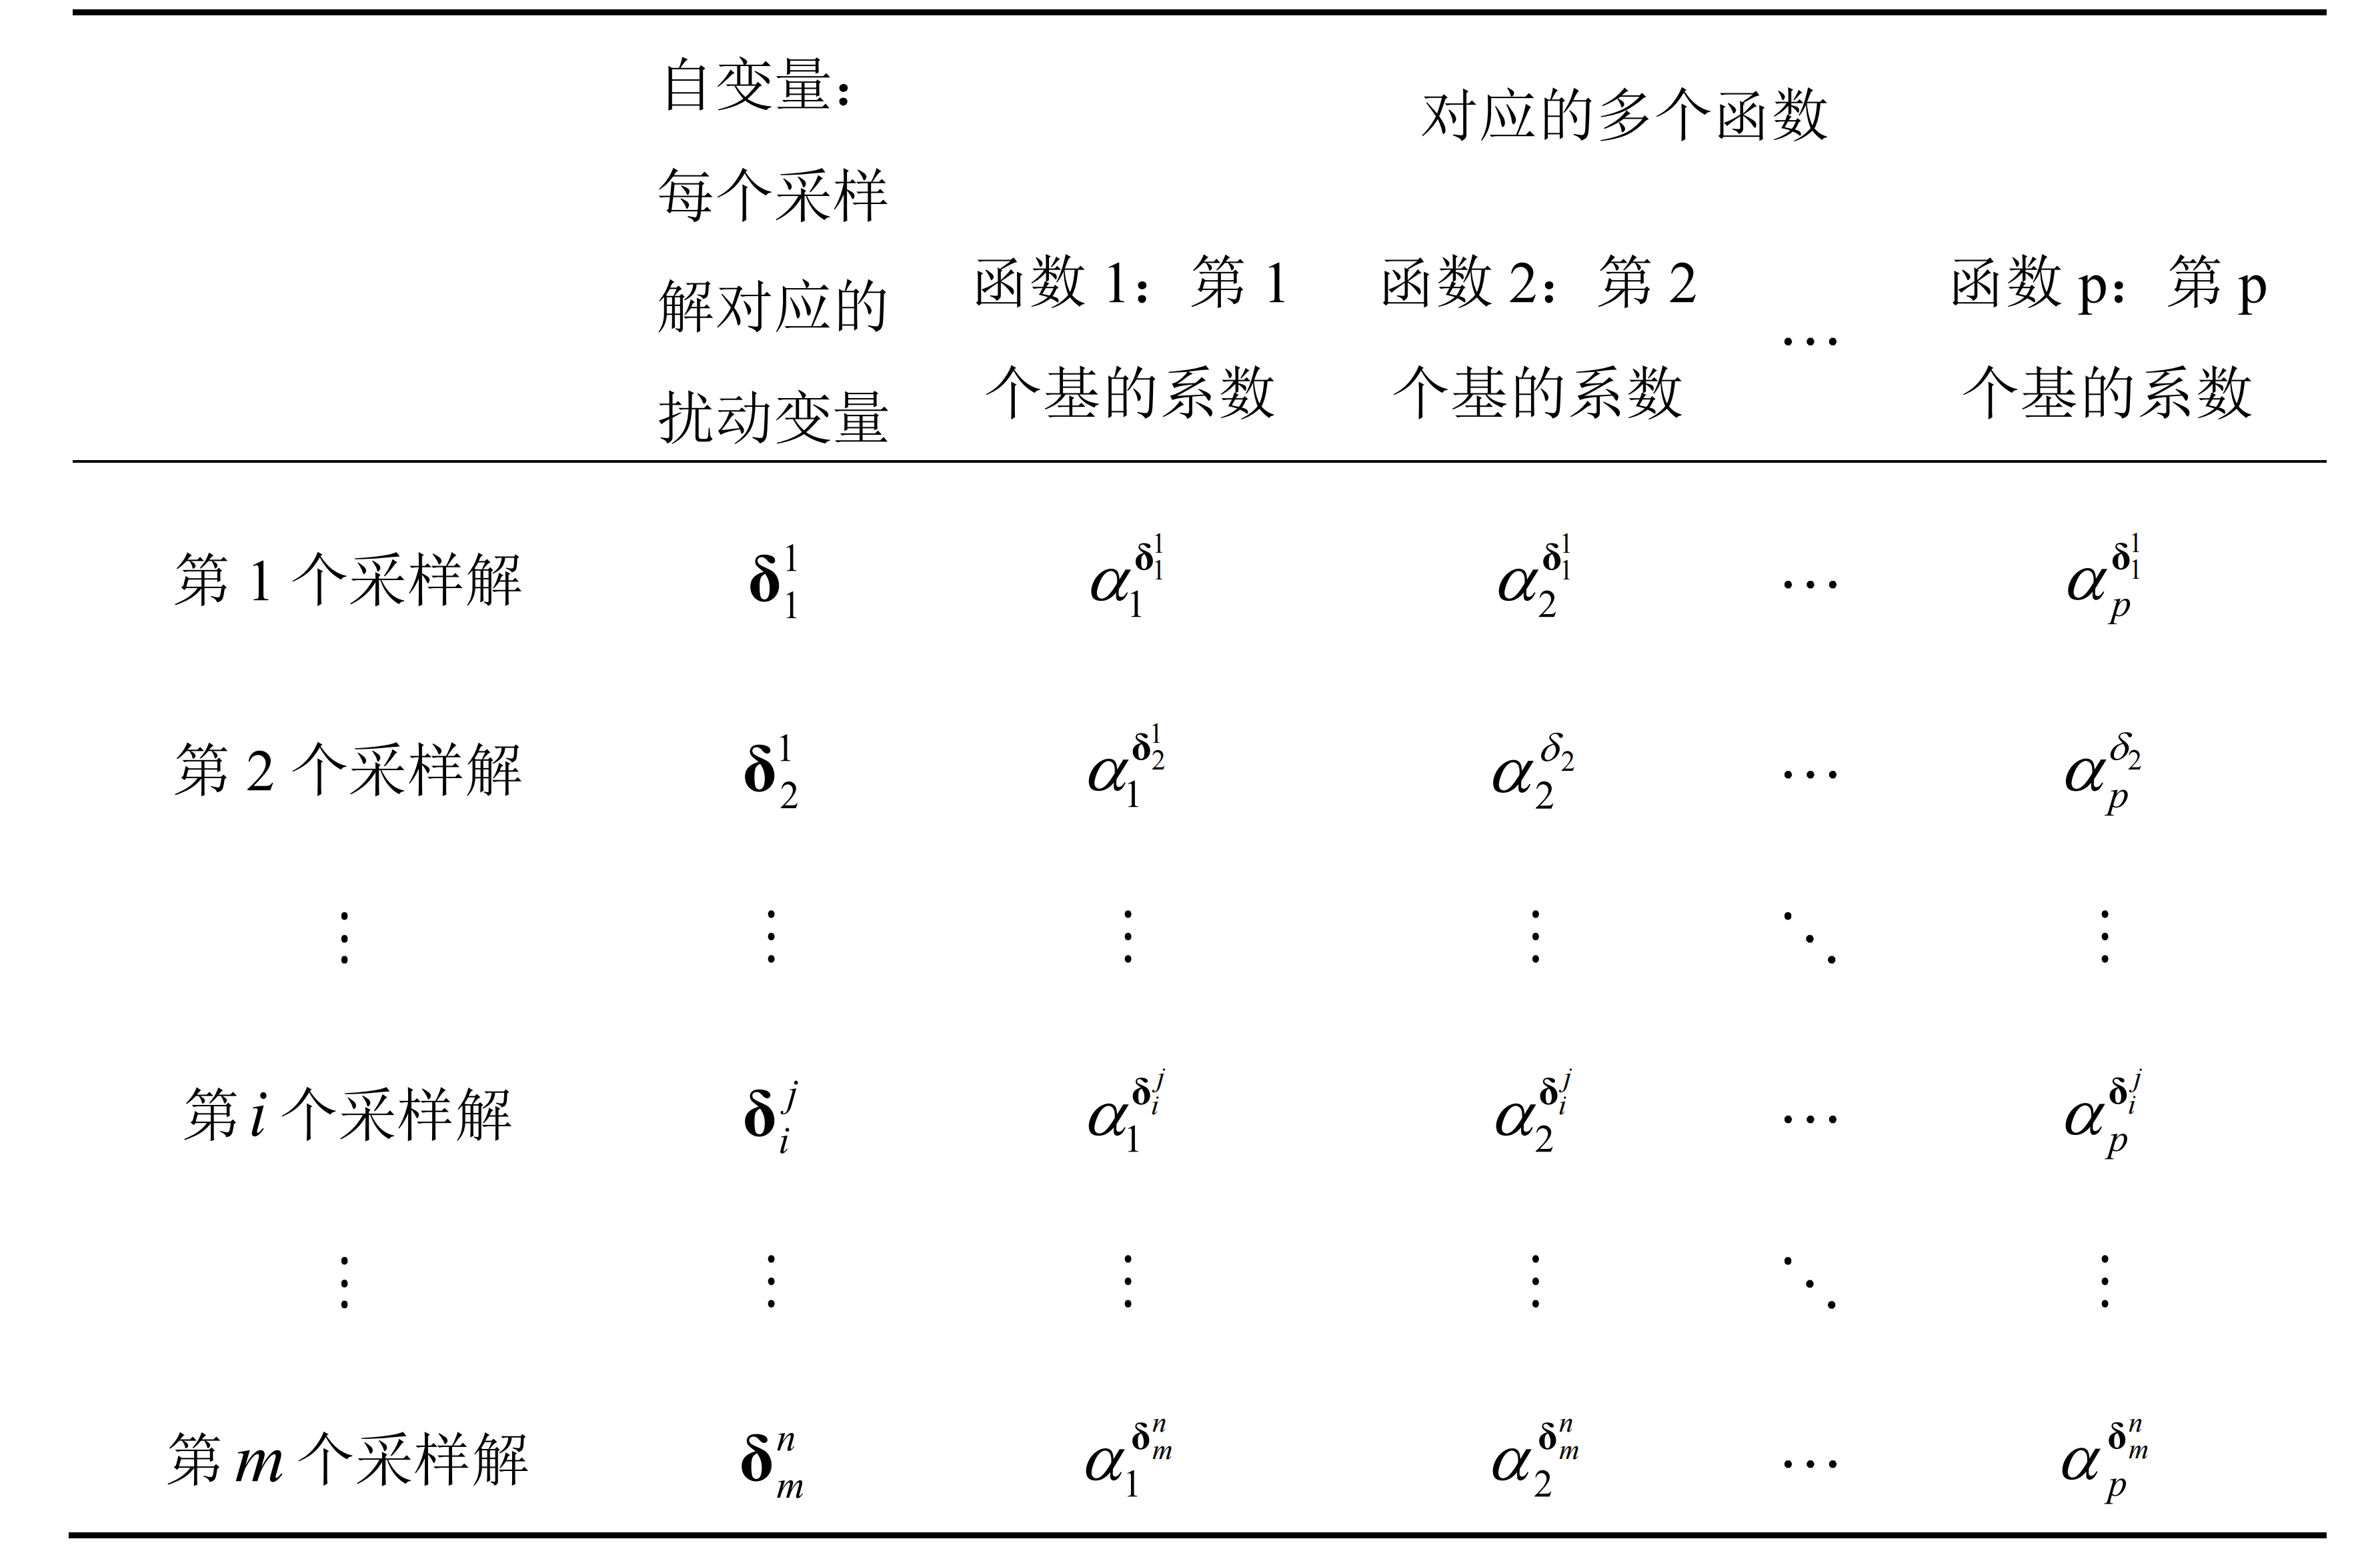
\includegraphics[width=1.0\linewidth]{自变量_00.png}
    \caption{\songti 插值关系表\\}
    \label{fig_result3}
\end{figure}
\section{单变量三次样条POD插值方法}
设参数变量为\(x\),为对于参数空间中的采样集 \(\{u^{(k)}\}_{k=1}^n\) 及其对应的POD降阶处理后的基矩阵 \(\{\Phi^{(k)}\}_{k=1}^m\)(保留前m个基),参数点 \(x\) 处的预测值\(u\)可表示为:
 \begin{equation}
    u(x) = \sum_{k=1}^{m} S_k(x) \Phi^{(k)}
    \end{equation}
其中\(S_k(x)\) 是满足 \(C^2\) 连续性的三次样条插值函数,用来表示待预测参数点\(x^*\)处对应的第k个POD基系数(共m个POD基,k的取值从1到m)。每个 \(S_k(x)\) 在子区间 \([x^{(i)}, x^{(i+1)}]\) 上的局部表达式为:
\begin{equation}
S_k^{(i)}(x) = a_k^{(i)} + b_k^{(i)} (x - x^{(i)}) + c_k^{(i)} (x - x^{(i)})^2 + d_k^{(i)} (x - x^{(i)})^3.
\end{equation}
通过求解三对角线性系统(自然边界条件)确定系数 \(\{a_k^{(i)}, b_k^{(i)}, c_k^{(i)}, d_k^{(i)}\}\)。

\begin{algorithm}[H]
\SetAlgoLined
\DontPrintSemicolon
\SetKwInOut{Input}{输入}
\SetKwInOut{Output}{输出}
\SetKwProg{Fn}{POD-Spline-Interpolation}{}{}
\SetAlFnt{\footnotesize}  % 缩小字体

\Input{
  快照矩阵 $\mathbf{U} \in \mathbb{R}^{n_d \times N}$ \quad
  参数采样点 $\{x^{(k)}\}_{k=1}^n$ \quad
  目标参数值 $x^*$
}
\Output{预测场 $\mathbf{u}_{rec} \in \mathbb{R}^{n_d}$}

\Fn{\POD-Spline-Interpolation{}}{
\Indp
  1. 计算POD模态:\\
  \quad $\triangleright$ 截断SVD分解:$[\mathbf{\Phi},\mathbf{\Sigma},\mathbf{V}] \gets \text{svds}(\mathbf{U}, m)$ \\
  \quad $\triangleright$ 能量验证:While $\sum_{i=1}^m \sigma_i^2/\sum \sigma_i^2 < 1-\epsilon$ do $m \gets m+1$ \;
  
  2. 投影系数计算:\\
  \quad \For{$k \gets 1$ \KwTo $n$}{
    $\boldsymbol{\alpha}^{(k)} \gets \mathbf{\Phi}^\top \mathbf{U}(:,k)$
  }\Indm
  
 \Indp
  3. 单变量样条构造:\\
  \For{$k \gets 1$ \KwTo $m$}{
    a. 生成三对角矩阵 $\mathbf{A}[i,j] = 
    \begin{cases}
      h_{i-1}/6, & j=i-1 \\
      (h_{i-1}+h_i)/3, & j=i \\
      h_i/6, & j=i+1
    \end{cases}$\; 
    b. 求解三对角系统:$\mathbf{c}_k \gets \text{ThomasSolver}(\mathbf{A}, \boldsymbol{\alpha}_k)$\;
  }
  
  4. 边界约束:\\
  \quad $\triangleright$ 自然边界条件 $S''(x_1) = S''(x_n) = 0$\;
  \quad $\triangleright$ 修正系统矩阵 $\mathbf{A}[1,1] \gets 1,\ \mathbf{A}[n,n] \gets 1$\;
  
  5. 重构预测场:\\
  \quad $\mathbf{u}_{rec} = \sum_{k=1}^m S_k(x^*)\boldsymbol{\phi}_k$\;
  \Indm
}
\caption{单变量三次样条POD插值算法}
\label{alg:pod_spline_1d}
\end{algorithm}
算法步骤:
\begin{enumerate}
  \item {POD基生成}:
在参数点集\(\{x^{k}\}_{k=1}^n\) 处采集样本数据,通过POD提取主模态m,生成基矩阵 \(\Phi^{}\)。

  \item{三次样条基函数构造}:
  对第\(k\)个POD基 ,构造三次样条函数 \(S_k(x)\)表示参数取值为x时第k个POD基的基系数,确保 \(C^2\) 连续性和自然边界条件(二阶导数为零)。

  \item {新参数插值}:
给定新参数值 \(x^*\),计算各基函数的基系数 \(S_k(x^*)\)。

  \item{合成预测值}:
 将POD基矩阵按权重线性组合,生成新参数下的预测函数:
    \[
    u(x) = \sum_{k=1}^{m} S_k(x) \Phi^{(k)}.
    \]
  \item{物理场重构}:使用插值后的预测值 \(u(x^*)\) 重构物理场。例如,网格点 \(i\) 的值为:
    \[
    \text{pod\_cubic}(i) = u(x^*)\ \cdot \text{pod\_basis}(i).
    \]
\end{enumerate}
\section{双变量三次样条POD插值方法}
单变量基函数在区间$[x_i,x_{i+1}]$上的局部表达式为:
\begin{equation}
    S_i(x) = \sum_{k=0}^3 a_k^{(i)}(x-x_i)^k
\end{equation}

通过张量积扩展,得到双变量样条函数表示为:
\begin{equation}
    S(x,y) = \sum_{i=1}^{m_x}\sum_{j=1}^{m_y} c_{ij}B_i^{(3)}(x)B_j^{(3)}(y)
\end{equation}

其中B样条基函数满足正交性:
\begin{equation}
    \int_{\Omega} B_i^{(3)}(x)B_j^{(3)}(x)dx = \delta_{ij}
\end{equation}
\subsection{低维系数插值}
对第$k$个POD模态系数场$\alpha_k(x,y)$构造样条:
\begin{equation}
    S_k(x,y) = \sum_{i=1}^{m_x}\sum_{j=1}^{m_y} c_{k,ij}B_i^{(3)}(x)B_j^{(3)}(y)
\end{equation}

插值条件为:
\begin{equation}
    S_k(x_p,y_q) = \alpha_k^{(p,q)},\quad \forall p\in[1,n_x],q\in[1,n_y]
\end{equation}

\subsection{方程求解}
全局方程组形式为:
\begin{equation}
    (\mathbf{A}_x \otimes \mathbf{A}_y)\mathbf{c} = \boldsymbol{\alpha}
\end{equation}

其中三对角矩阵$\mathbf{A}_x$的元素为:
\begin{equation}
    a_{ij} = \begin{cases}
        \frac{h_{i-1}}{6}, & j=i-1 \\
        \frac{h_{i-1}+h_i}{3}, & j=i \\
        \frac{h_i}{6}, & j=i+1
    \end{cases}
\end{equation}

\subsection{边界条件处理}
修正自然边界条件:
\begin{equation}
    \sum_{k=1}^r \left.\frac{\partial^2 \phi_k}{\partial x^2}\right|_{x=x_b} \alpha_k(x,y) = 0 \quad (x_b \in \{x_0,x_n\})
\end{equation}

通过Lagrange乘子法扩展方程组:
\begin{equation}
    \begin{bmatrix}
        \mathbf{K} & \mathbf{G}^T \\
        \mathbf{G} & \mathbf{0}
    \end{bmatrix}
    \begin{bmatrix}
        \mathbf{c} \\
        \boldsymbol{\lambda}
    \end{bmatrix}
    =
    \begin{bmatrix}
        \boldsymbol{\alpha} \\
        \mathbf{0}
    \end{bmatrix}
\end{equation}
\subsection{算法关键步骤说明}
\begin{enumerate}
    \item{三对角矩阵求解}:采用Thomas算法,时间复杂度$\mathcal{O}(n)$,实现如下:
    \begin{align}
        &c'_1 \leftarrow c_1 / b_1 \nonumber\\
        &d'_1 \leftarrow d_1 / b_1 \nonumber\\
        &\text{For } i=2 \text{ to } n-1: \nonumber\\
        &\quad c'_i \leftarrow \frac{c_i}{b_i - a_i c'_{i-1}} \nonumber\\
        &\quad d'_i \leftarrow \frac{d_i - a_i d'_{i-1}}{b_i - a_i c'_{i-1}} \nonumber\\
        &M_n \leftarrow d'_n \nonumber\\
        &\text{For } i=n-1 \text{ downto } 1: \nonumber\\
        &\quad M_i \leftarrow d'_i - c'_i M_{i+1}
    \end{align}

    \item{Kronecker积加速}:利用矩阵分解特性降低计算复杂度:
    \begin{equation}
        (\mathbf{A} \otimes \mathbf{B})^{-1} = \mathbf{A}^{-1} \otimes \mathbf{B}^{-1}
    \end{equation}

    \item{边界处理优化}:引入快速投影法处理非齐次边界条件:
    \begin{equation}
        \mathbf{c} \leftarrow \mathbf{c} - \mathbf{G}^T(\mathbf{G}\mathbf{G}^T)^{-1}\mathbf{G}\mathbf{c}
    \end{equation}
\end{enumerate}
\begin{algorithm}[H]
\SetAlgoLined
\DontPrintSemicolon
\SetKwInOut{Input}{输入}
\SetKwInOut{Output}{输出}
\SetKwProg{Fn}{POD-Spline-Interpolation}{}{}
\SetAlFnt{\footnotesize}  % 缩小字体

\Input{
  快照矩阵 $\mathbf{U} \in \mathbb{R}^{n_d \times N}$ \quad
  参数网格 $\{(x_i,y_j)\}_{i,j=1}^{n_x,n_y}$ \quad
  目标点 $(x^*,y^*)$
}
\Output{重构场 $\mathbf{u}_{rec} \in \mathbb{R}^{n_d}$}

\Fn{\POD-Spline-Interpolation{}}{
\Indp
  1. 计算POD模态:\\
  \quad $\triangleright$ 截断SVD分解:$[\mathbf{\Phi},\mathbf{\Sigma},\mathbf{V}] \gets \text{svds}(\mathbf{U}, r)$ \\
  \quad $\triangleright$ 能量验证:While $\sum_{i=1}^r \sigma_i^2/\sum \sigma_i^2 < 1-\epsilon$ do $r \gets r+1$ \;
  
  2. 投影系数计算:\\
  \quad \For{$i \gets 1$ \KwTo $n_x$}{
    \For{$j \gets 1$ \KwTo $n_y$}{
      $\boldsymbol{\alpha}^{(i,j)} \gets \mathbf{\Phi}^\top \mathbf{U}(:,i,j)$
    }
  }\Indm
  
 \Indp
  3. 双变量样条构造(并行执行):\\
  \For{$k \gets 1$ \KwTo $r$}{
    a. 生成三对角矩阵 $\mathbf{A}_x[i,j] = 
    \begin{cases}
      h_{i-1}/6, & j=i-1 \\
      (h_{i-1}+h_i)/3, & j=i \\
      h_i/6, & j=i+1
    \end{cases}$\; 
    b. 计算 $\mathbf{K} = \mathbf{A}_x \otimes \mathbf{A}_y$\; 
    c. 求解 $\mathbf{c}_k \gets \text{ThomasSolver}(\mathbf{K}, \boldsymbol{\alpha}_k)$\;
  }
  
  4. 边界约束:构造 $\mathbf{G} = \left[\frac{\partial^2 \phi_k}{\partial x^2}\big|_{x=x_b}\right]$\\
  求解 $\begin{bmatrix}
    \mathbf{K} & \mathbf{G}^\top \\ \mathbf{G} & \mathbf{0}
  \end{bmatrix}
  \begin{bmatrix}
    \mathbf{c} \\ \boldsymbol{\lambda}
  \end{bmatrix} = 
  \begin{bmatrix}
    \boldsymbol{\alpha} \\ \mathbf{0}
  \end{bmatrix}$\;
  
  5. 重构场 $\mathbf{u}_{rec} = \sum_{k=1}^r S_k(x^*,y^*)\boldsymbol{\phi}_k$\;
  \Indm
}
\caption{POD双变量三次样条插值算法}
\label{alg:pod_spline_compact}
\end{algorithm}



\section{Kriging 模型理论}
Kriging 函数模型由回归模型与相关模型相加而成,其形式为\cite{JTKJ201904016}:
\begin{equation}
    y(x) = f(x)^T \beta + z(x)
    \label{eq:2.1}
\end{equation}

式中:\( f(x) \) 为多项式模型(回归模型),根据需求可以选择零阶、一阶、二阶多项式,其表达式为:
\begin{equation}
    f(x)^T \beta = [f_1(x), f_2(x), \ldots, f_p(x)] \beta = f_1(x) \beta_1 + f_2(x) \beta_2 + \cdots + f_p(x) \beta_p
    \label{eq:2.2}
\end{equation}
式中:\( p \) —— 多项式数量;

\quad\( \beta \) —— 线性回归系数的向量;

\quad\( z(x) \) —— 被假定为遵循 \( (0, \sigma^2) \) 正态分布,并且是一个数学期望为 0、标准偏差为 \( \sigma \) 的随机过程(相关模型)。

在Kriging模型的构建中,参数化部分的作用等同于多项式部分,主要负责实现模型的全局拟合功能。由于Kriging模型具有确定性输出的特性,即相同的输入参数总是产生相同的响应输出,因此多项式部分与响应之间的误差主要来源于建模误差本身,这种误差对模型整体拟合精度的影响相对较小。基于此,通常在建立Kriging模型时,将\( f(x) \) 设定为零阶多项式。此时的Kriging模型被命名为普通Kriging模型,其变量满足二阶平稳性假设。

二阶平稳假定:

(1)随机过程 \( z(x) \) 的数学期望是一个确定的常数:
\begin{equation}
    E[z(x)] = a
    \label{eq:2.3}
\end{equation}

(2)区域化变量 \( z(x) \) 的协方差函数存在并且相等:
\begin{align}
    Cov[z(x), z(x+h)] &= E[(z(x) - E[z(x)])(z(x+h) - E[z(x+h)])] \notag \\
    &= E[z(x)z(x+h)] - E[z(x)]E[z(x+h)] \notag \\
    &= E[z(x)z(x+h)] - a^2 \notag \\
    &= Cov(h)
    \label{eq:2.4}
\end{align}

对区域化变量 \( z(x) \),Kriging模型能够有效捕捉结构输入参数与输出响应之间的非线性关系,从而显著提高响应面的拟合精度。在估计 \( z(x) \)时,Kriging模型需要假设响应面是连续的,并且预测点的响应仅与空间距离相关 \( z(x) \)的协方差矩阵为:
\begin{equation}
    Cov[z(x_i), z(x_j)] = \sigma^2 R[R(x_i, x_j)]
    \label{eq:2.5}
\end{equation}
式中:\( R \) —— 相关矩阵,对于拟合高精度的Kriging模型起到主要作用; 

\quad\( R(x_i, x_j) \) —— 两个样本点 \( x_i, x_j \) 之间的空间相关函数。其函数形式见表3.1。
\begin{table}[htbp]
    \centering
    \caption{相关矩阵 \( R(x_i, x_j) \) 的函数形式}
    \label{tab:2.1}
    \begin{tabular}{ll}
        \toprule
        相关函数 &\hspace{2cm} \(\quad R(x_i, x_j) \) \\
        \midrule
        高斯函数 &\hspace{2cm} \(   \exp(-\theta_s|d_s|) \) \\
        指数函数 &\hspace{2cm} \(   \exp(-\theta_sd_s^2) \) \\
        线性函数 &\hspace{2cm} \(   \max\{0, 1 - \theta_s|d_s|\} \) \\
        球形函数 &\hspace{2cm} \(   1 - 1.5\xi_s + 0.5\xi_s^3 \quad\qquad\qquad\qquad\xi_s = \min \{1, \theta_s |d_s|\}\) \\
        三次函数 &\hspace{2cm} \(   1 - 3\xi_s^2 + 2\xi_s^3 \ \ \qquad\qquad\qquad\qquad\xi_s = \min \{1, \theta_s |d_s|\}\) \\
        样条函数 &\hspace{1cm} 
        \( \varsigma(\xi_s) = \begin{cases}
            1 - 15\xi_s^2 + 30\xi_s^3, & 0 \leq \xi_s \leq 0.2 \\
            1.25(1 - \xi_s)^3, & 0.2 < \xi_s < 1\qquad\xi_s=\theta_s |d_s| \\
            \qquad0,&\quad\xi_s \geq1
        \end{cases} \) \\
        \bottomrule
    \end{tabular}
    \begin{tablenotes}
        \item 注:1. 表中 \( d_s = |x_i^s - x_j^s| \),\( x_i^s \)、\(x_j^s \) 分别为两个样本点的第 \( s \) 个分量;
        \item 2. \( \theta_s \) 为特征值参数,控制不同维度上相关性的衰减率。
    \end{tablenotes}
\end{table}

样本点之间的相关函数矩阵为:
\begin{equation}
\mathrm{R}= \begin{bmatrix} R(x_1,x_1) & \cdots & R(x_1,x_n) \\ \vdots & \ddots & \vdots \\ R(x_n,x_1) & \cdots & R(x_n,x_n) \end{bmatrix}
\end{equation}

样本的似然函数表达式为:
\begin{equation}
    L = \frac{1}{(2\pi\sigma^2)^{m/2}|R|^{1/2}} \exp\left[-\frac{(Y-F\beta)^T R^{-1}(Y-F\beta)}{2\sigma^2}\right]
    \label{eq:2.7}
\end{equation}
式中:
F——每个样本点的向量$f(x)$的矩阵;

\quad Y——每个响应向量$y(x)$的矩阵;
 
\quad$m$——设计变量的数量。

根据最大似然估计法可得:
\begin{align}
    \hat{\beta} &= (F^T R^{-1} F)^{-1} F^T R^{-1} Y
    \label{eq:2.8} \\
    \hat{\sigma}^2 &= \frac{(Y-F\hat{\beta})^T R^{-1} (Y-F\hat{\beta})}{n}
    \label{eq:2.9} 
\end{align}

最大似然函数的对数表达式为:
\begin{align}
\ln(L) = -\frac{n}{2} \ln(2\pi) - \frac{n}{2} \ln(\hat{\sigma}^2) - \frac{1}{2} \ln |R|
\end{align}

通过求解最大似然函数的最大值,可以确定不同维度上的待估计参数 $\theta_s$ 的值。

基于上述公式,Kriging模型中关于已知样本点与响应之间的关系已经建立。接下来,我们将对未知点的响应进行预测。假设对于任意点,其预测值能够最大化样本点与预测点之间的增广似然函数,可以通过公式(3.22)来计算未知点的响应预测值:
未知点响应预测值为:
\begin{equation}
    \hat{y}(x_0) = f(x_0)^T \hat{\beta} + r(x_0)^T R^{-1} (Y-F\hat{\beta})
    \label{eq:3.22}
\end{equation}

通过式(3.23)可以获取预测值的均方差,进行响应面的精度验算:
\begin{equation}
   \hat{s}(x)^2=\sigma^2\left[1-\{f(x)^T,r(x)^T\}\left[ \begin{array} {cc}0 & \mathrm{F}^T \\ \mathrm{F} & \mathrm{R} \end{array}\right]^{-1}\left\{ \begin{array} {c}f(x) \\ r(x) \end{array}\right\}\right]
    \label{eq:3.23}
\end{equation}
式中:$\mathbf{r(x_0)^T}$ —— 预测点和样本点之间的相关函数的行向量,表达式为:
\begin{equation}
\mathbf{r(x_0)^T} = [R(x_0, x_1), ..., R(x_0, x_n)]
\end{equation}

当预测第 $i$ 个样本点时,因为 $\mathbf{r(x_i)^T R^{-1}}$ 等于第 $i$ 阶单位向量,式(3.22)可写为:
\begin{equation}
    \hat{y}(x_i) = f(x_i)^T \hat{\beta} + y_i - f(x_i)^T \hat{\beta} = y_i
    \label{eq:2.14}
\end{equation}

式(3.25)说明 Kriging 模型对于未知点的响应预测值与实际响应值相等,故 Kriging
模型可以代替有限元模型进行分析计算。 \cite{1025273058.nh}
\section{误差分析方法}
\label{sec:4.1}
为系统评估插值POD方法的流场重构性能,本研究采用定量误差分析与相关性验证相结合的评价体系。具体通过以下三类指标实现:

\begin{itemize}
    \item {均方根误差(RMSE)}:反映局部大误差分布特征
    \begin{equation}
        \text{RMSE} = \sqrt{\frac{1}{n} \sum_{i=1}^{n} \left( y_i^{\text{pred}} - y_i^{\text{true}} \right)^2}
        \label{eq:rmse}
    \end{equation}

    \item{平均绝对误差(MAE)}:表征全局误差水平
    \begin{equation}
        \text{MAE} = \frac{1}{n} \sum_{i=1}^{n} \left| y_i^{\text{pred}} - y_i^{\text{true}} \right|
        \label{eq:mae}
    \end{equation}

    \item{皮尔逊相关系数(Pearson's $r$)}:评估趋势一致性
    \begin{equation}
        r = \frac{\sum_{i=1}^{n} (y_i^{\text{pred}} - \bar{y}^{\text{pred}})(y_i^{\text{true}} - \bar{y}^{\text{true}})}
        {\sqrt{\sum_{i=1}^{n} (y_i^{\text{pred}} - \bar{y}^{\text{pred}})^2 \sum_{i=1}^{n} (y_i^{\text{true}} - \bar{y}^{\text{true}})^2}}
        \label{eq:pearson}
    \end{equation}
\end{itemize}

%缺少两个图片

% Overleaf\footnote{网址可见\url{https://www.overleaf.com/}}是一个在线的Latex文档协作平台。我们不需要配置任何环境,便能够在上面直接使用本模板进行写作。操作步骤如下:

% 第一步,下载本项目压缩包(从\url{https://github.com/SYSU-SCC/sysu-thesis/releases}处下载即可),注意需要下载zip格式的压缩包。
% 然后,我们在Overleaf上新建项目,并上传该压缩包,可参考\autoref{fig:overleaf-new-proj}。


% \begin{figure}[h]
% 	\centering
% 	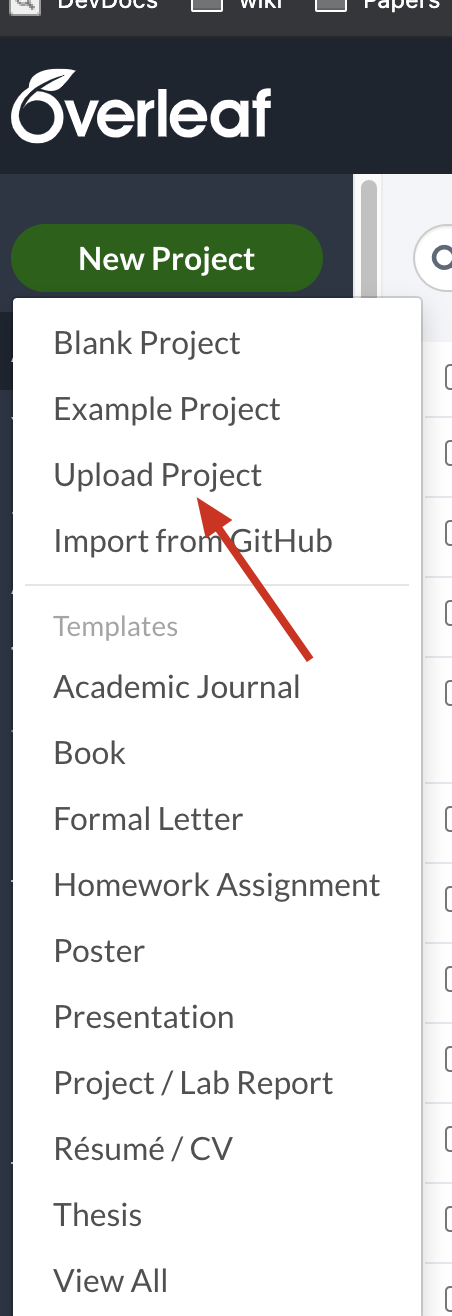
\includegraphics[width=0.2\textwidth]{image/chap03/overleaf-create-proj.jpg}
% 	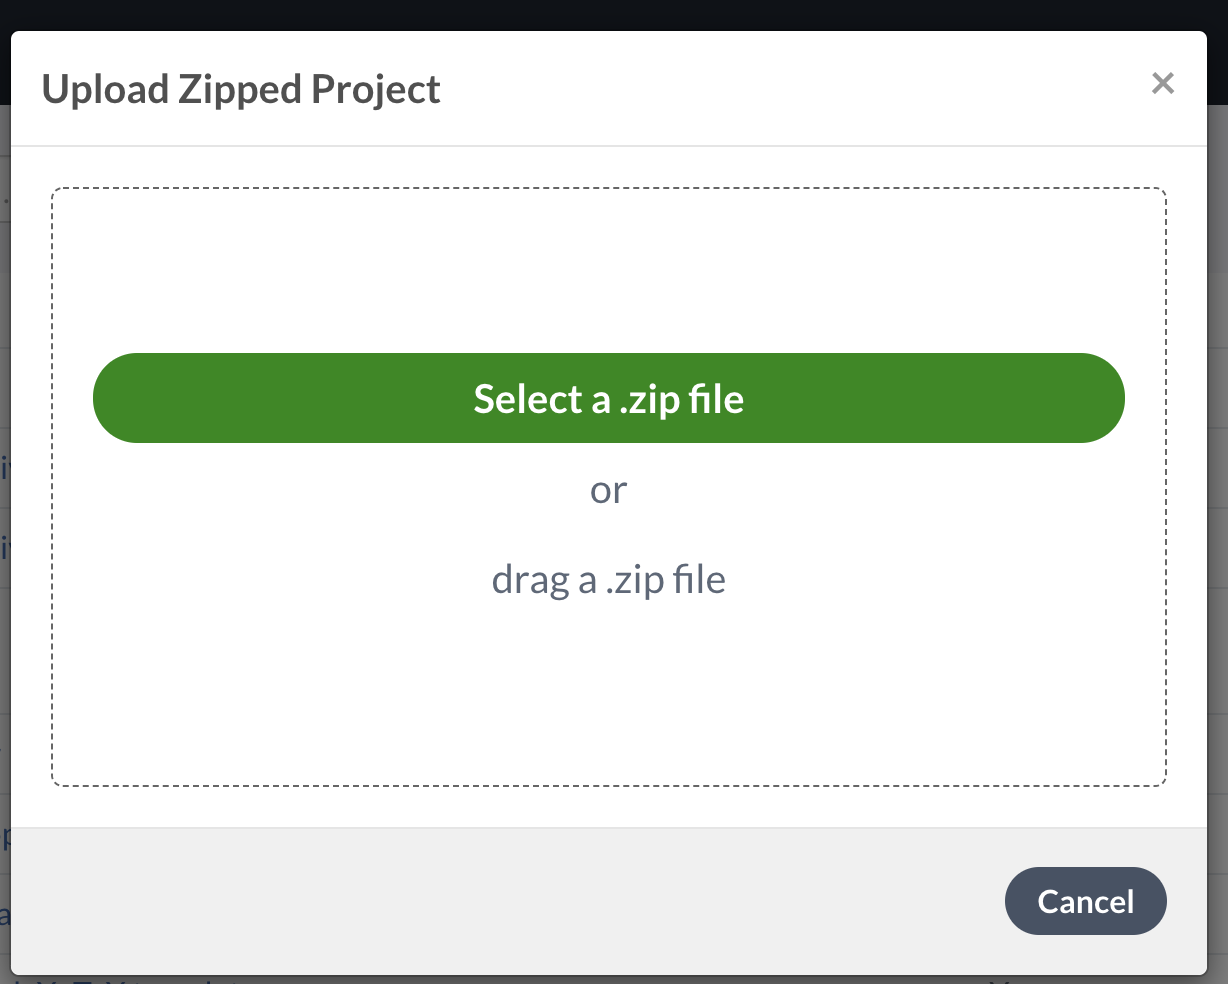
\includegraphics[width=0.7\textwidth]{image/chap03/overleaf-upload-proj.jpg}
% 	\caption{在Overleaf上创建并上传压缩包。}
% 	\label{fig:overleaf-new-proj}
% \end{figure}

% 第二步,在Overleaf的菜单中调整编译工具为\texttt{xelatex},可参考\autoref{fig:overleaf-config}。

% \begin{figure}[h]
% 	\centering
% 	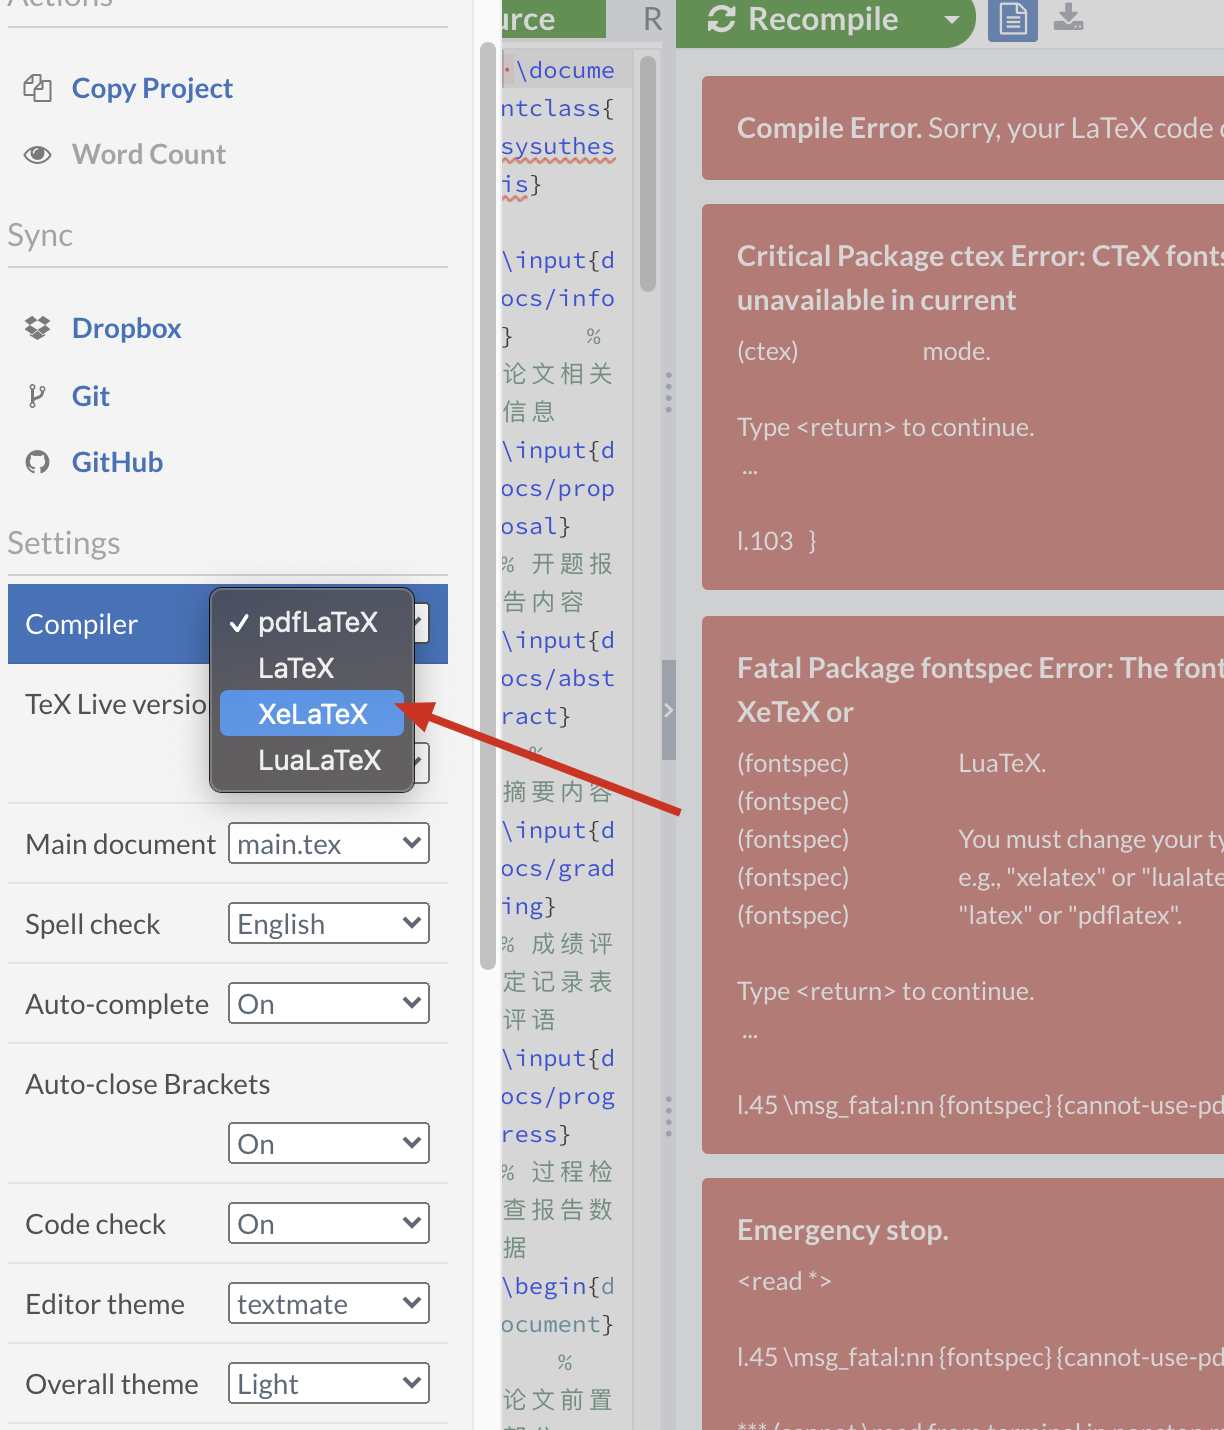
\includegraphics[width=0.6\textwidth]{image/chap03/overleaf-config.jpg}
% 	\caption{在Overleaf上调整编译工具}
% 	\label{fig:overleaf-config}
% \end{figure}


% 第三步,点击编译,得到本pdf,可以开始修改pdf了!最终可见\autoref{fig:overleaf-example}。


% \begin{figure}[h]
% 	\centering
% 	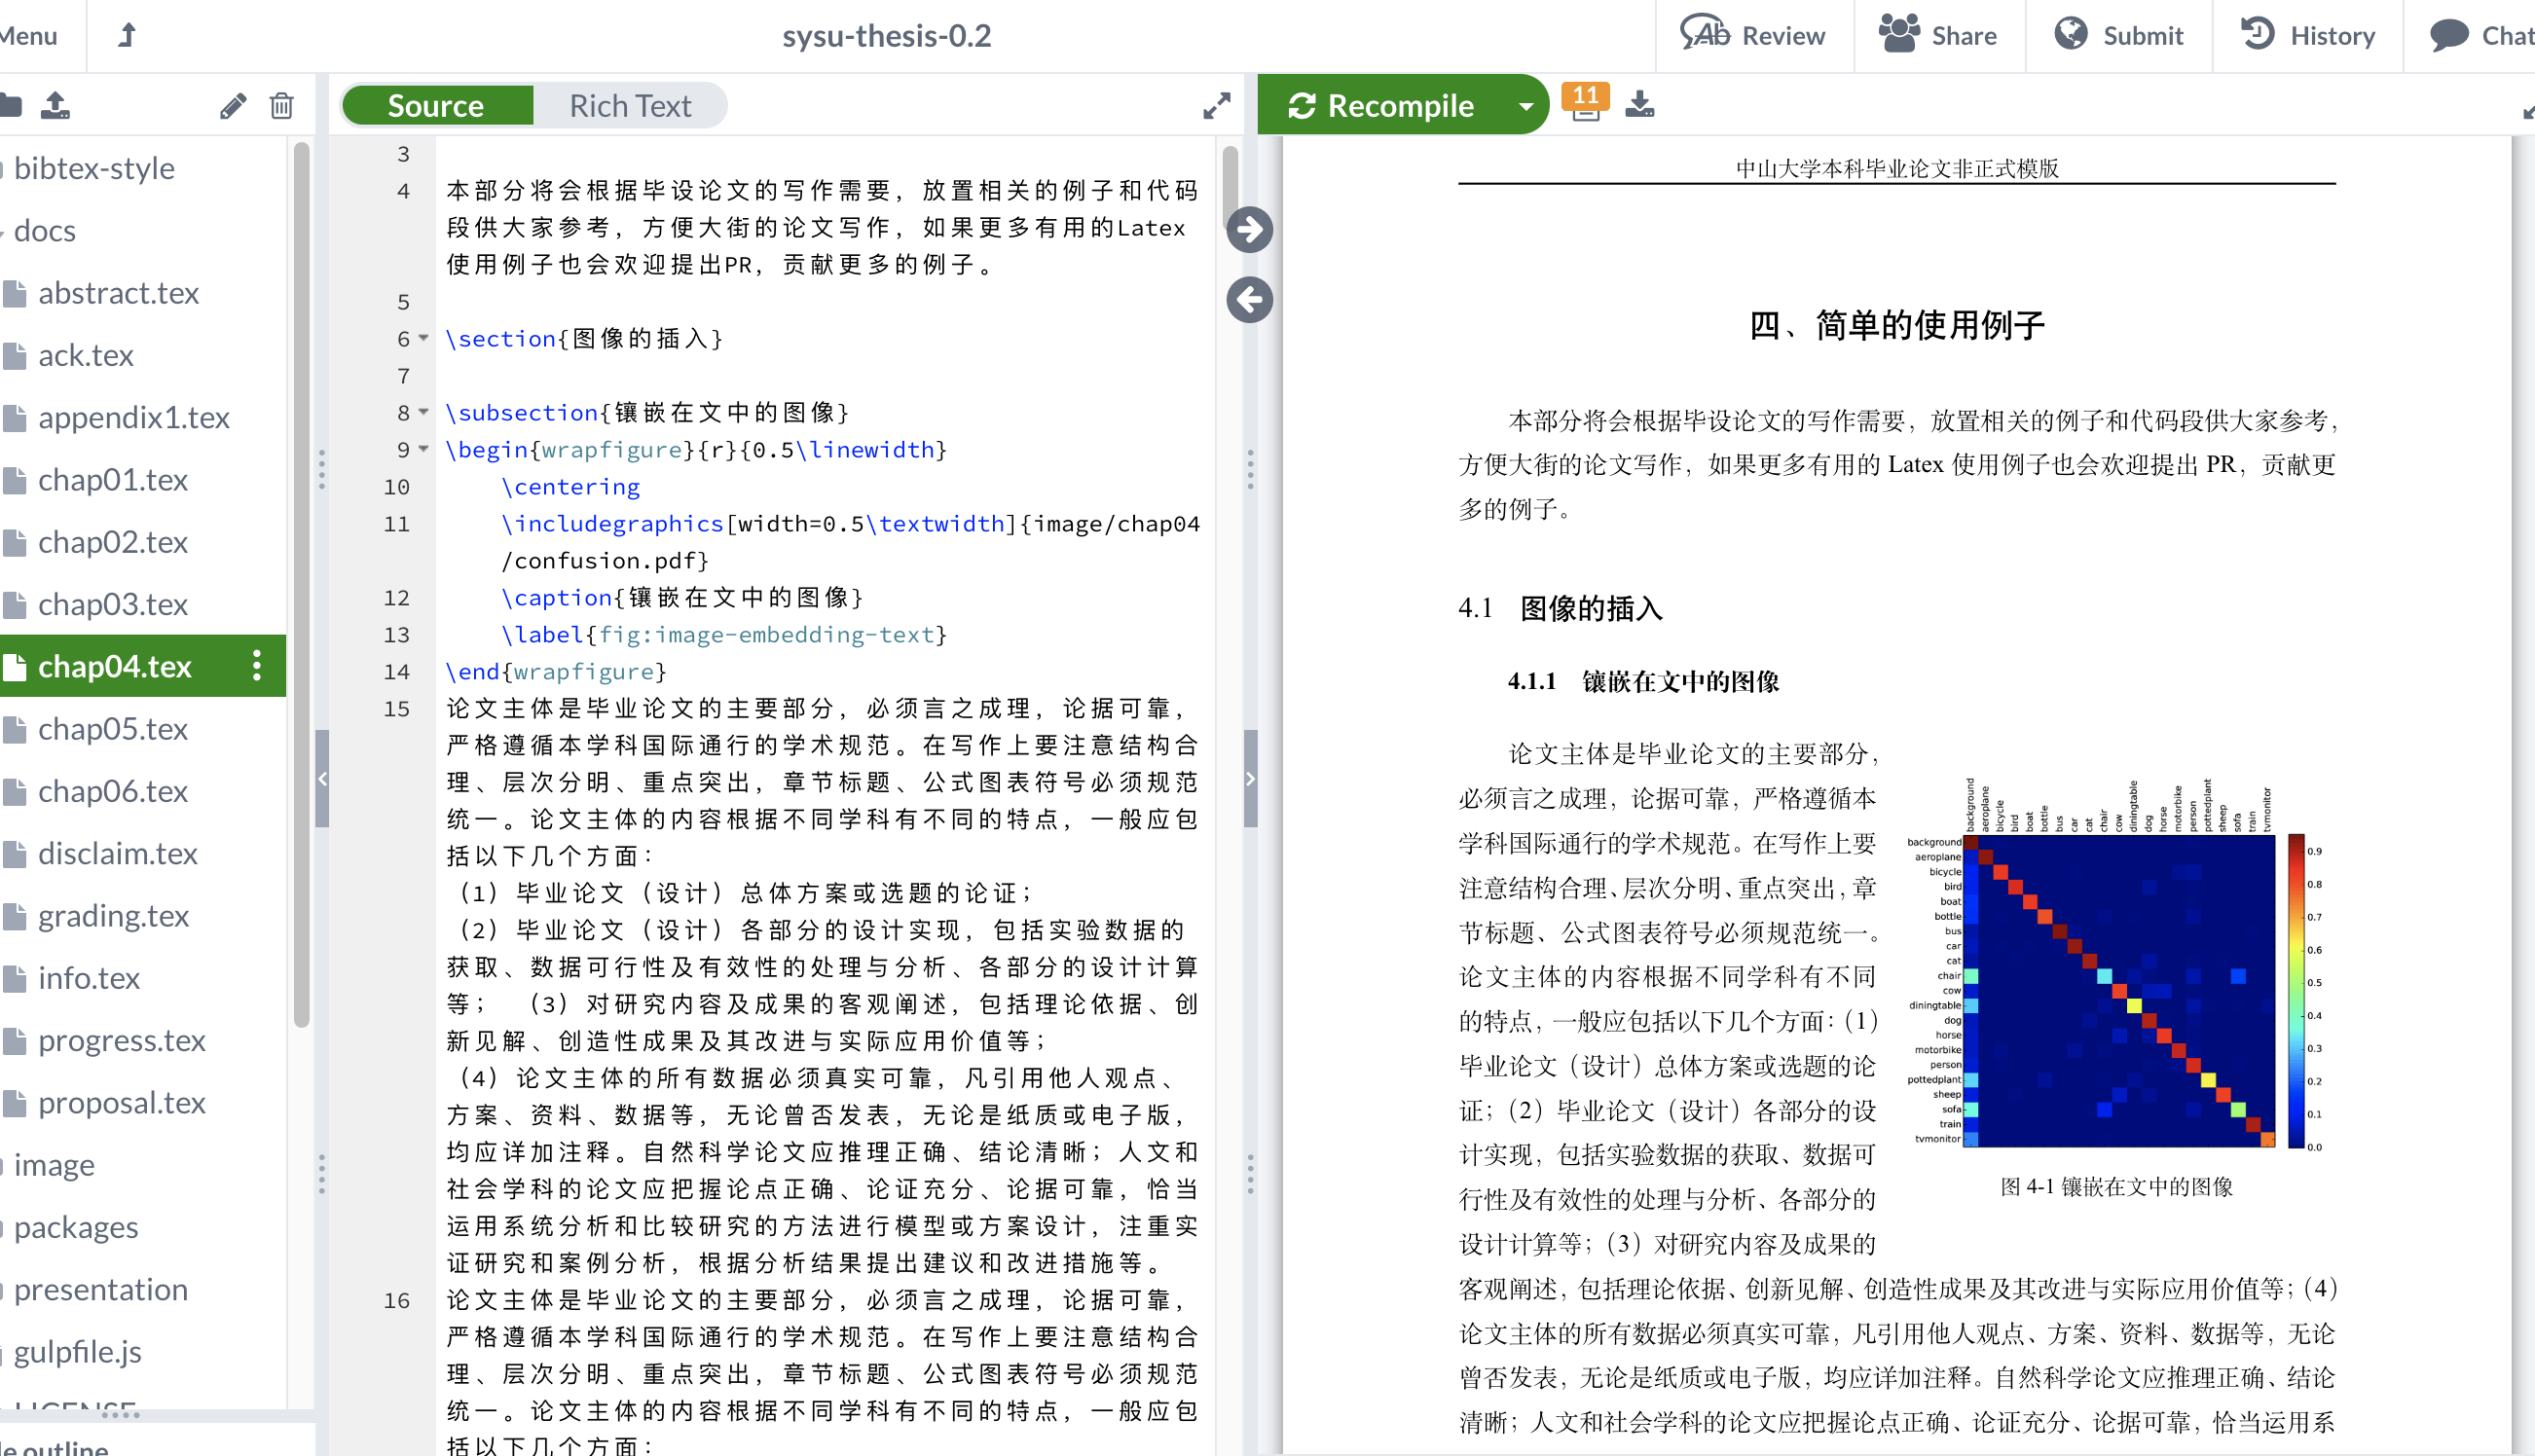
\includegraphics[width=0.9\textwidth]{image/chap03/overleaf-example.jpg}
% 	\caption{Overleaf使用例子}
% 	\label{fig:overleaf-example}
% \end{figure}



%\section{编译环境配置}

% 编译环境配置相对来说比较简单,下载Tex Live2020并如同一般的程序一样安装即可。

% \subsection{编译环境配置:Window篇}

% 在\url{https://mirrors.tuna.tsinghua.edu.cn/CTAN/systems/texlive/Images/}上下载Tex Live2020并参考教程\footnote{可以参考\url{https://zhuanlan.zhihu.com/p/58811994}}安装即可。

% \subsection{编译环境配置:Linux篇}

% 在\url{https://mirrors.tuna.tsinghua.edu.cn/CTAN/systems/texlive/Images/}上下载Tex Live2020并参考教程\footnote{可以参考\url{https://zhuanlan.zhihu.com/p/55894177}}安装即可。


% \subsection{编译环境配置:MacOS篇}

% 在MacOS上配置Latex的环境,这里我们使用的是MacTex。

% \begin{enumerate}
% 	\item \url{https://www.tug.org/mactex/}下载MacTex安装。
% 	\item 安装步骤:不详细展开,按照图形界面点击即可, 傻瓜式安装。
% \end{enumerate}

% TIPS:MacTex文件比较大,有2G多,介意的话可以选择MacTex\_Basic包,只有100M以内,但是如果安装MacTex\_Basic,后期可能会遇到各种缺包的问题。


% 安装完成之后,可以简单测试一下安装是否成功。如可以查看Texshop应用是否安装好,或者在命令行测试一下\texttt{xelatex}命令是否可用。

%\section{写作环境配置}

% 不同的写作工具对应不同的写作环境。这里我们给出几个工具的配置例子以供参考。

% \subsection{模板编译流程}

% 由于\LaTeX 的限制,本模板需要经过四次编译才能生成完整的论文:

% \begin{enumerate}
% 	\item 先使用xelatex编译一次
% 	\item 再使用bibtex编译一次
% 	\item 然后使用xelatex编译两次
% \end{enumerate}

% 本编译流程已经写在Makefile中,修改模板源码后只需要执行\texttt{make pdf}即可按照该流程进行编译并生成最终的pdf。



% \subsection{写作环境配置:Visual Studio Code}

% Visual Studio Code是微软公司推出的轻量代码编辑器,我们可以做一些简单的配置,便可以用该编辑器修改我们的\LaTeX 模板,并实现一键编译。

% \begin{enumerate}
% 	\item 安装 Visual Studio Code。
% 	\item 安装 LaTeX Workshop 插件。
% \end{enumerate}

% 本项目的\texttt{.vscode/setting.json}下已经包含了与前面所述编译流程相同的配置。正常配置下,每次修改模板源码后按下保存(Ctrl+S),就能够自动进行编译产生pdf。效果图如\autoref{fig:vscode-example}所示。


% \begin{figure}[h]
% 	\centering
% 	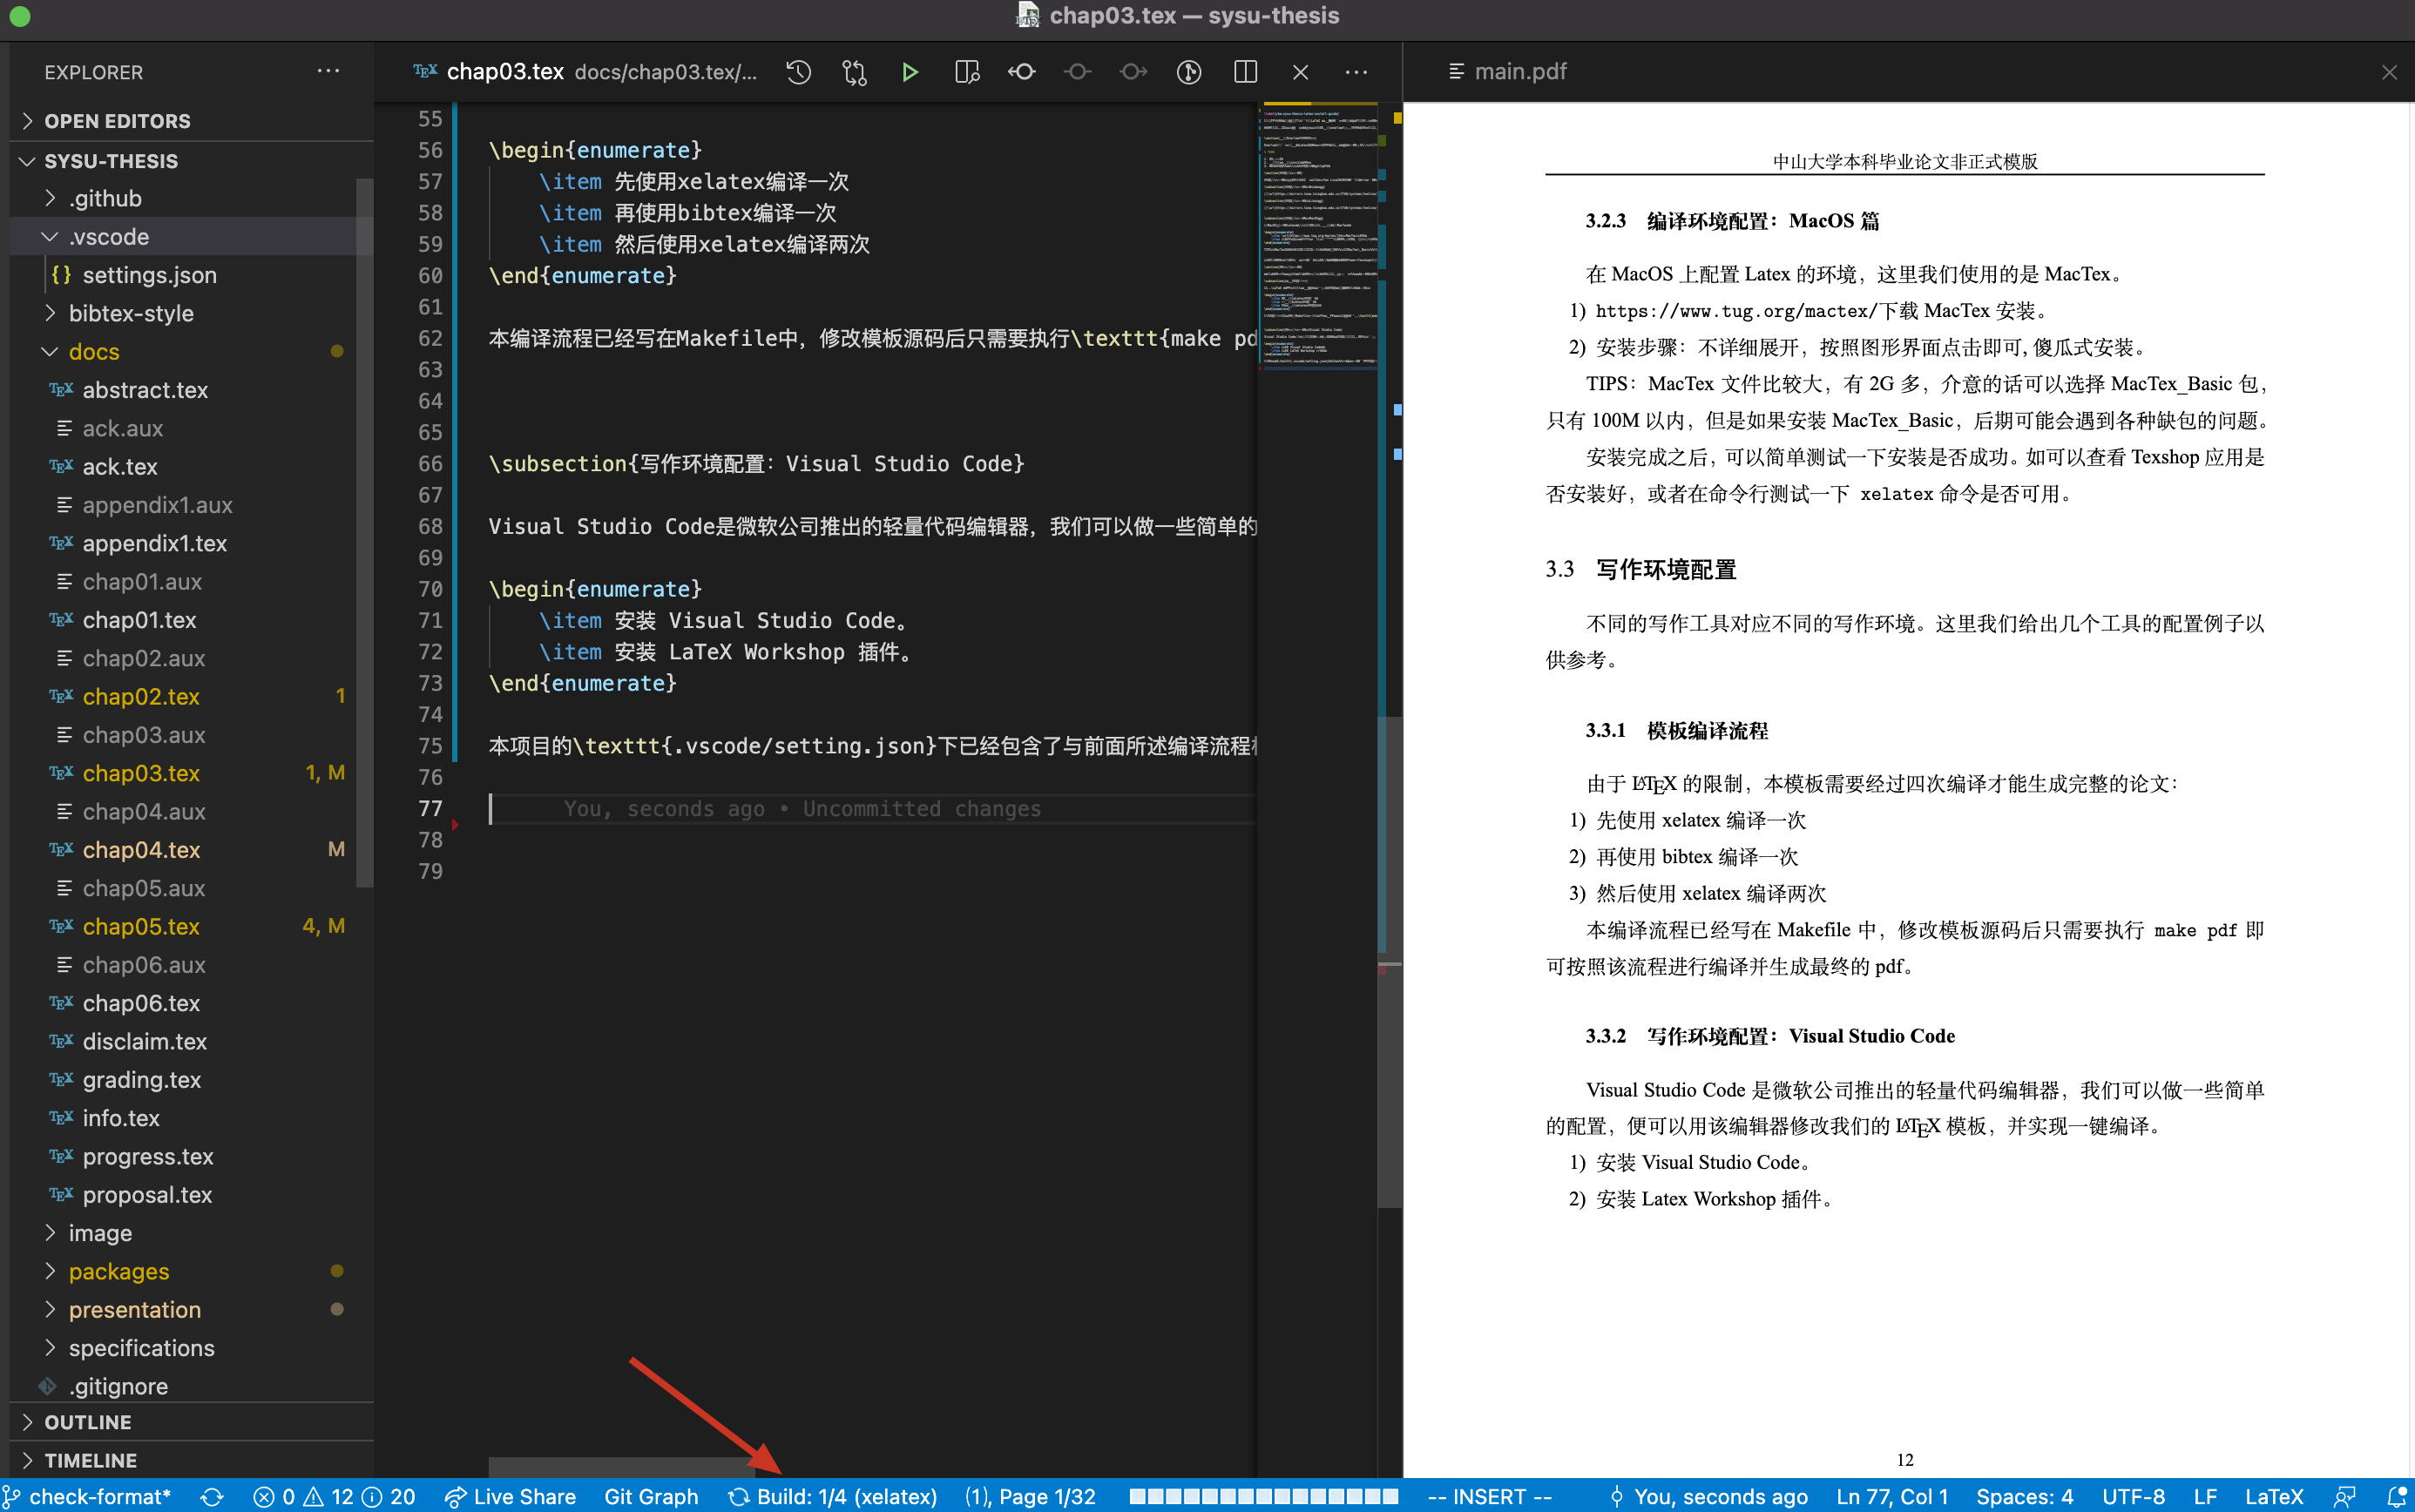
\includegraphics[width=\linewidth]{image/chap03/vscode-example.png}
% 	\caption{vscode配置好后的样例}
% 	\label{fig:vscode-example}
% \end{figure}


%\section{如何开始写毕业论文(设计)}

% 首先将所有个人信息,包括学号、姓名、专业、论文题目等,在\texttt{./docs/info.tex}中逐项进行更新。

% 然后我们再编辑\texttt{./docs/abstract.tex}补充论文摘要。

% 到了论文主体部分,我们可以自行编辑\texttt{./docs/chap01.tex},\texttt{./docs/chap02.tex}等文件进行编辑。如果章数不够,可以自行修改\texttt{main.tex}增加新的章节。

% 当论文主体编写完成后,我们再编辑\texttt{./docs/ack.tex}作为论文致谢。


% 首先将个人信息写到\texttt{./docs/info.tex}中。